\documentclass[english]{beamer}
\usepackage[utf8]{inputenc}
\usepackage[english]{babel}
\usepackage{multicol}
\usepackage{tikz}

\usetheme[language=english,footline=sections,faculty=tw,usecolors,framenumber,totalframenumber]{UniversiteitGent}

\usetikzlibrary{arrows}
\usetikzlibrary{fit}
\usetikzlibrary{calc}
\usetikzlibrary{backgrounds}
\usetikzlibrary{shapes.geometric}
\usetikzlibrary{positioning}
\tikzset{hide on/.code={\only<#1>{\color{white}}}}
\tikzset{
	invisible/.style={opacity=0},
	visible on/.style={alt=#1{}{invisible}},
	alt/.code args={<#1>#2#3}{%
		\alt<#1>{\pgfkeysalso{#2}}{\pgfkeysalso{#3}} % \pgfkeysalso doesn't change the path
	},
	level/.style={sibling distance = 4cm/#1,level distance = 1.5cm},
	treenode/.style = {align=center, inner sep=0pt, text centered,
		font=\ttfamily},
	arn_l/.style = {treenode, circle, ugentblue, draw=ugentblue, fill=ugentyellow,
		text width=1.5em, very thick},% leaf node
	arn_x/.style = {treenode, circle, white, draw=ugentblue, fill=ugent-pp,
		text width=1.5em, very thick},% red
	arn_y/.style = {treenode, circle, white, draw=ugentblue, fill=ugent-tw,
		text width=1.5em, very thick},% blue
	arn_0/.style = {treenode, draw=none,
		fill=none, text width=0},% hidden node
	arn_s/.style = {treenode, circle,
		fill=ugentblue, text width=0.75em},%small node
	rect_l/.style ={shape=rectangle, rounded corners, draw, align=center,
		color=ugentblue, top color=ugentyellow, bottom color=ugentyellow, very thick},
	rect_x/.style ={shape=rectangle, rounded corners, draw, align=center,
		color=ugentblue, top color=ugent-pp, bottom color=ugent-pp, very thick},
}


\AtBeginSection[]
{
	\begin{frame}<beamer>
		\begin{multicols}{2}
			\tableofcontents[currentsection,hideothersubsections]
		\end{multicols}
	\end{frame}
}


\title{Design of a diagnosis and follow-up platform for patients with chronic headaches}
%\subtitle{Phylogeny Comparison}
\author{Kiani Lannoye \& Gilles Vandewiele}
\mode<beamer>{\institute{Faculty of Engineering and Architecture}}

\begin{document}
\begin{frame}
	\titlepage
\end{frame}

\section{Intro}
\label{sec:intro}
\begin{frame}{Introduction}
	\framesubtitle{test}
	\begin{figure}[!h]
		\centering
		
\includegraphics[width=\textwidth]{figures/headache.jpg}
	\end{figure}
\end{frame}

\begin{frame}{Headaches}
	\begin{figure}[!h]
		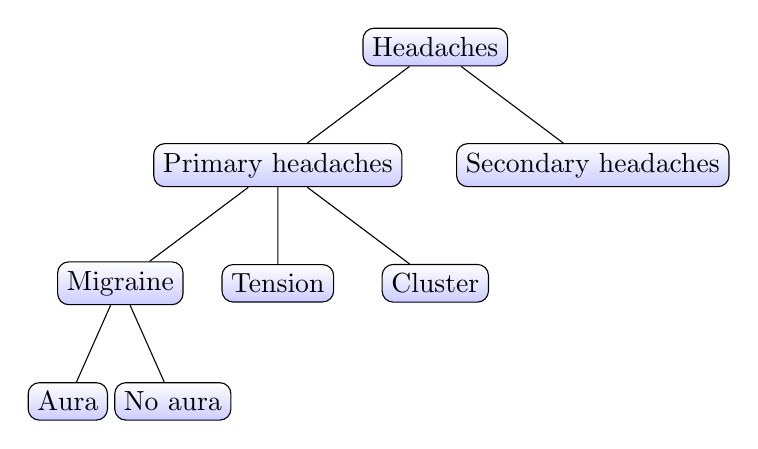
\begin{tikzpicture}[sibling distance=10em,
		every node/.style = {shape=rectangle, rounded corners,
			draw, align=center,
			top color=white, bottom color=blue!20}]]
		\only<5>{}
		\node {Headaches}
		child[visible on=<2->] { 
			node {Primary headaches} 
				child[visible on=<4->] {
					node {Migraine}
						child[visible on=<5->] {
							node {Aura}
						}
						child[visible on=<5->]{
							node {No aura}
						}
				}
				child[visible on=<4->] {
					node {Tension}
				}
				child[visible on=<4->] {
					node {Cluster}
				}
		}
		child[visible on=<3->] { node {Secondary headaches}};
		\end{tikzpicture}
		\caption{Headaches overview}
	\end{figure}
\end{frame}


% section intro (end)
\section{Platform requirements}
\label{sec:simMess}
% section Platform requirements (end)
\section{Mobile application}
\section{Backend and data exposure}
\section{Machine learning - decision trees}

\subsection*{Why decision trees?}

\subsection*{Decision tree induction algorithms}

\subsection*{Ensemble techniques}

\section{Genetic merging of decision trees}
\subsection*{Introduction}

\begin{frame}{Many different induction algorithms}
	\begin{itemize}
		\item QUEST
		\item CART
		\item C4.5 (C5.0)
		\item $\ldots$
	\end{itemize} \vspace{2em}
	\textbf{$\rightarrow$ Which one is the best?}
\end{frame}

\begin{frame}{Current ensembles lack interpretability}
	\begin{block}{}
	\textbf{Boosting, bagging, random forests,} etc. require majority voting (classification) or mean calculation (regression) to obtain prediction
	\end{block}
	
	\vspace{3em}
	\resizebox{0.24\textwidth}{!}{%
	\begin{tikzpicture}
	\node (A) [arn_l] {};
	\node (B) [arn_l, below left=0.75cm and 0.75 cm of A] {};
	\node (C) [arn_l, below right=0.75cm and 0.75 cm of A] {};
	\node (D) [rect_l, below left of=B] {0};
	\node (E) [rect_l, below right of=B] {1};
	\node (F) [rect_l, below left of=C] {1};
	\node (G) [rect_x, below right of=C] {0};
	\draw (A) -- (B);
	\draw (A) -- (C);
	\draw (B) -- (D);
	\draw (B) -- (E);
	\draw (C) -- (F);
	\draw (C) -- (G);
	\end{tikzpicture}%
	 } \resizebox{0.24\textwidth}{!}{%
		\begin{tikzpicture}
		\node (A) [arn_l] {};
		\node (B) [arn_l, below left=0.75cm and 0.75 cm of A] {};
		\node (C) [arn_l, below right=0.75cm and 0.75 cm of A] {};
		\node (D) [rect_l, below left of=B] {0};
		\node (E) [rect_l, below right of=B] {1};
		\node (F) [rect_l, below left of=C] {1};
		\node (G) [rect_x, below right of=C] {0};
		\draw (A) -- (B);
		\draw (A) -- (C);
		\draw (B) -- (D);
		\draw (B) -- (E);
		\draw (C) -- (F);
		\draw (C) -- (G);
		\end{tikzpicture}%
		 } \resizebox{0.24\textwidth}{!}{ %		
	 	$\ldots$ %
		}	\resizebox{0.24\textwidth}{!}{%
		\begin{tikzpicture}
		\node (A) [arn_l] {};
		\node (B) [arn_l, below left=0.75cm and 0.75 cm of A] {};
		\node (C) [arn_l, below right=0.75cm and 0.75 cm of A] {};
		\node (D) [rect_l, below left of=B] {0};
		\node (E) [rect_x, below right of=B] {1};
		\node (F) [rect_l, below left of=C] {1};
		\node (G) [rect_l, below right of=C] {0};
		\draw (A) -- (B);
		\draw (A) -- (C);
		\draw (B) -- (D);
		\draw (B) -- (E);
		\draw (C) -- (F);
		\draw (C) -- (G);
		\end{tikzpicture}%
		 }
	
	\framesubtitle{Stacking}
\end{frame}

\begin{frame}{Current ensembles lack interpretability}
	\begin{block}{}
		The final decision tree obtained by \textbf{stacking} contains uninterpretable internal nodes
	\end{block}
	
	\vspace{2em}
	
	\begin{tikzpicture}
	\centering
	\node (A) [rect_l] {$x_1 \leq 5.0$};
	\node (B) [rect_x, below left=0.75cm and 0.75 cm of A] {$outcome_{NN} \leq 2.0$};
	\node (C) [rect_x, below right=0.75cm and 0.75 cm of A] {$outcome_{RF} \leq 4.0$};
	\node (D) [rect_l, below left=0.5cm and 0.5cm of B] {0};
	\node (E) [rect_l, below right=0.5cm and 0.5cm of B] {1};
	\node (F) [rect_l, below left=0.5cm and 0.5cm of C] {0};
	\node (G) [rect_l, below right=0.5cm and 0.5cm of C] {1};
	\draw (A) -- (B);
	\draw (A) -- (C);
	\draw (B) -- (D);
	\draw (B) -- (E);
	\draw (C) -- (F);
	\draw (C) -- (G);
	\end{tikzpicture}
	
\end{frame}

\subsection*{Merging different decision trees}

\subsection*{Genetic algorithm}
\section{Visualization - doctor dashboard}
\section{Conclusion \& future work}




% subsection rstar (end)

% section concensusTeees (end)

\begin{frame}<beamer> 
  \frametitle{Bedankt}
	  {\huge \color{ugentyellow} Bedank voor uw aandacht}\\
	  No written word,
	  
	  No spoken plea,
	  
	  Can teach the youth what they should be,
	  
	  Nor all the books on all the shelves,
	  
	  It's what the teachers are themselves 
\end{frame}

\begin{frame}<beamer> 
	\small
	\tableofcontents
\end{frame}
\end{document}